\chapter{Particles II (Application)} % (fold)
\label{cha:particles II (Application)}
\section{Photon and Phonon} % (fold)
\label{sec:photon_and_phonon}
\subsection{黑体辐射} % (fold)
\label{sub:黑体辐射}
\begin{definition}[黑体\index{黑体}]
    黑体,指的是能够完全吸收任何波长的外来辐射而无任何反射的物体。
\end{definition}

理想的黑体当然是不存在的,实验上可以用一个开了小孔的金属空腔来近似黑体(这里的黑体指的是这个孔,不是金属空腔本身)。

对于特定体积的容器$V$是固定的,由于我们只考察平衡态的情形,因此该体系需要与环境达成热平衡,即$T$一定。但是由于器壁会不断地吸收和释放光子,因此$N$是无法确定的。

\begin{remark}
    由于不同的电磁波之间发生直接转化,只能通过物质的吸收和发生来间接转化。因此表征物质转化趋势的化学势$\mu$在这里是没有意义的。所以我们直接取$\mu=0$。
\end{remark}

在进一步讨论之前,我们可以稍微回顾一下光子最重要也是最基本的性质——波粒二象性。

\subsubsection{波动性描述}

\begin{table}[h]
    \centering
    \begin{tabular}{cccccc}
        周期$T$ & 频率$\nu$ & 角频率 $\omega =2\pi \nu$ & 波长$\lambda$ & 波数$\widetilde{\nu}=\frac{1}{\lambda}$ & 波矢 $k=2\pi \widetilde{\nu}$ \\
    \end{tabular}
\end{table}

以及最关键的公式\begin{equation}
    \lambda \nu =c
\end{equation}
空间中的一个平面波可以表示为\begin{equation}
    \varphi=A\left[e^{i(\bd{k} \cdot \bd{r}-\omega t)}+\text{C.C.}\right]
\end{equation}

\subsubsection{粒子性描述}

光子的能量和动量分别为 \begin{equation}
    E=h\nu=\hbar \widetilde{\nu}, \quad \bd{p}=h\bd{k}
\end{equation}
利用平面波色散关系\begin{equation}
    \omega=ck
\end{equation}
就可以得到能量-动量关系\begin{equation}
    E=pc
\end{equation}

在光子气模型中$N$没有办法确定,因此$\mu$是没有意义的,我们的分析只能立足于$V,T$。这个时候巨正则配分函数和正则配分函数等价\begin{equation}
    \Xi =Q
\end{equation}

对于一个微观态$v$,它可以用不同的状态以及占据数来描述\begin{equation}
    v\leftrightarrow \{\omega_i , \bd{k}_i, g_i, n_i\}
\end{equation}
其中$\omega_i$,$\bd{k}_i$,$g_i$,$n_i$分别是频率、波矢、振动模式、占据数,由于光子是玻色子,所以$n_i$可以取任意自然数。微观态$v$的能量可以表示为\begin{equation}
    E_v=\sum_i n_i \hbar\omega_i
\end{equation}

我们知道,对于玻色子其配分函数为\begin{equation}
    \ln \Xi =-\sum_i \ln (1-e^{-\beta \varepsilon_i}),\quad (\mu=0)
\end{equation}
以及某一个能级的占据数\begin{equation}
    \braket{n_i}=\frac{1}{e^{\beta\varepsilon_i}-1}
\end{equation}
将这个结果应用于光子气,就有\begin{equation}
    \braket{E} =-\diffp{\ln \Xi}{\beta} =\sum_i \braket{n_i} \varepsilon_i=\sum_i \frac{\varepsilon_i}{e^{\beta\varepsilon_i}-1}
\end{equation}
其中$\varepsilon_i =n_i\hbar\omega_i$
实际的频率应该近似为一个连续分布,于是求和可以化成积分\begin{equation}
    \braket{E} =\int_0^\infty \frac{\varepsilon}{e^{\beta\varepsilon}-1} \rho(\varepsilon)\di\varepsilon
\end{equation}

\begin{remark}
    如果我们想要知道黑体的某一个能量区间中的光子密度,只需要知道这个态对应的驻波的种类数。一维情形下驻波的条件为\begin{equation}
        a=n\cdot \frac{\lambda}{2}
    \end{equation}
    所以\begin{equation}
        k=\frac{2\pi}{\lambda} =\frac{n\pi}{a}
    \end{equation}
    这个结论可以拓展到三维,于是就有\begin{equation}
        \bd{k}=\frac{\pi}{a} (n_x \bd{i}+n_y\bd{j}+n_z\bd{k})
    \end{equation}
    或者\begin{equation}
        k^2 =\frac{\pi^2}{a^2} (n_x^2+n_y^2+n_z^2)
    \end{equation}
    注意到\begin{equation}
        k=\frac{\omega}{c} =\frac{\varepsilon}{\hbar c}
    \end{equation}
    于是\begin{equation}
        n_x^2+n_y^2+n_z^2 =\frac{\varepsilon^2 a}{\pi\hbar^2 c^2} 
    \end{equation}
    因此能量介于$0\sim \varepsilon$之间的态的数量就等于\begin{equation}
        2\times\frac{1}{8} \times \frac{4}{3} \pi \left(\frac{\varepsilon}{\hbar c\pi}\right)^3=\frac{V}{6\pi^2} \frac{\varepsilon^3}{\hbar^3 c^3}
    \end{equation}
    上式中的因子2来自于偏振自由度,于是\begin{equation}
        \rho(\varepsilon) =\di\left(\frac{V}{3\pi^2} \frac{\varepsilon^3}{\hbar^3 c^3} \right) =\frac{V}{\pi^2}\frac{\varepsilon^2}{\hbar^3c^3} \di\varepsilon
    \end{equation}
\end{remark}

据此我们就可以进一步计算平均能量\begin{equation}
    \braket{E} =\int_{0}^{+\infty}\frac{V}{\pi^2}\frac{\varepsilon^2}{\hbar^3c^3} \frac{\varepsilon}{e^{\beta\varepsilon}-1}\mathrm{d}\varepsilon
\end{equation}
因为$\varepsilon=\hbar \omega$,所以\begin{equation}
    \braket{E} =\int_{0}^{+\infty}\frac{V}{\pi^2 c^3 }\frac{\hbar\omega^3}{e^{\beta\hbar\omega}-1} \mathrm{d}\omega
\end{equation}
其中\begin{equation}
    p_{T,V} =\frac{V}{\pi^2c^3} \frac{\hbar\omega^3}{e^{\beta \hbar\omega}-1}
\end{equation}
被称为黑体辐射的普朗克公式\index{黑体辐射的普朗克公式}。在此基础上,我们可以进行一些更加细致的分析。

对于高温低频的情形,$\displaystyle \frac{\hbar \omega}{kT}\ll 1$,整理后有\begin{equation}
    p_{T,V}=kT \omega^2 \frac{V}{\pi^2 c^3}
\end{equation}
这个公式被称为Rayleigh-Jeans公式,\index{Rayleigh-Jeans公式},此时主要表现为波动性。

对于低温高频的情形,$\displaystyle \frac{\hbar \omega}{kT}\gg 1$,整理后有\begin{equation}
    p_{T,V}=\frac{V}{\pi^2 c^3}\hbar \omega^3 e^{-\frac{\hbar \omega}{kT}}
\end{equation}
被称为Wien公式\index{Wien公式},其图形如图\ref{fig:wien equation}。这个时候主要表现为粒子性。不难发现$\omega_{\max}\propto T$,即黑体辐射谱的峰值位置只和温度有关,我们称之为Wien位移定律\index{Wien位移定律}。
\begin{figure}[h]
       \centering
       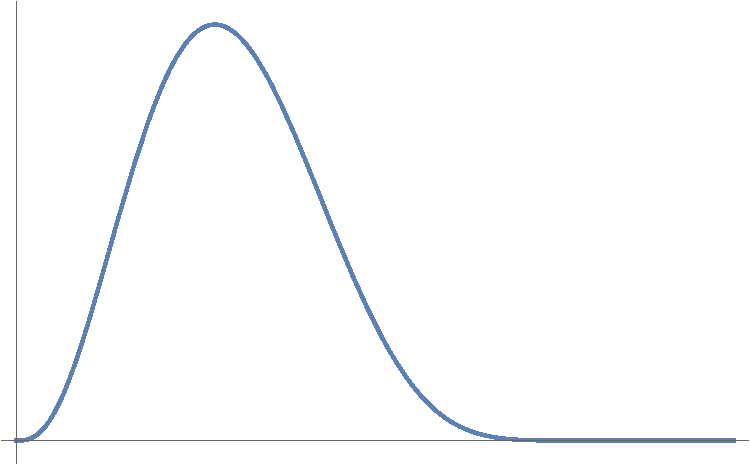
\includegraphics[width=0.6\textwidth]{fig/wien.pdf}
       \caption{黑体辐射的Wien公式}
       \label{fig:wien equation}
\end{figure}

重新考虑我们之前得到的$\braket{E}$,\begin{equation}
    \braket{E} =\frac{8\pi V}{h^2 c^3} \int_0^{+\infty} \frac{\varepsilon^3}{e^{\beta \varepsilon}-1}\di \varepsilon
\end{equation}
所以体积能量密度\begin{equation}
    \frac{\braket{E}}{V} = \frac{8\pi}{h^3 c^3 \beta^4} \int_0^{+\infty} \frac{x^3}{e^x -1} \di x=\frac{8\pi^5}{15h^3 c^3} (kT)^4
\end{equation}

考虑这个体系的配分函数,就有\begin{equation}
\begin{aligned}
    \ln \Xi &=-\sum_i \ln\left(1-e^{-\beta\varepsilon_i}\right)\\
    &= -\int_{0}^{+\infty}\ln (1-e^{-\beta \varepsilon} ) \rho(\varepsilon) \mathrm{d}\varepsilon\\
    & = -\int_{0}^{+\infty} \ln (1-e^{-\beta \varepsilon} )  \frac{8\pi v}{h^3 c^3}\varepsilon^2\mathrm{d}\varepsilon\\
    & = -\frac{8\pi V}{\beta^3 h^3 c^3} \int_{0}^{+\infty}\ln(1-e^{-x})x^2  \mathrm{d}x=-\frac{1}{3} \frac{8\pi^5 v \beta^{-3}}{45 h^3 c63}
\end{aligned}
\end{equation}

在配分函数的基础上,我们可以回顾一下之前的物理量:\begin{gather}
    \braket{E} = -\diffp{{\ln \Xi}}{{\beta}} =\frac{8\pi^5 V}{15h^3 c^3}(kT)^4\\
    p=\frac{kT}{V} \ln \Xi =\frac{8\pi^5}{45h^3 c^3}\beta^{-4}
\end{gather}
特别地,这里有\begin{equation}
    pV =\frac{1}{3}\braket{E}
\end{equation}

考虑到$\mu=0$,因此熵满足\begin{equation}
    S=k\ln \Xi +\frac{\braket{E}}{T} =4k\ln\Xi
\end{equation}
以及\begin{equation}
    A=E-TS =-kT \ln \Xi
\end{equation}
% subsection 黑体辐射 (end)
\subsection{声子} % (fold)
\label{sub:声子}
在金属晶体中,我们认为金属正离子在晶格位置附近振动,而电子弥散在电子海中。实验中我们观察到晶体的热容满足如下的规律:
\begin{figure}[h]
       \centering
       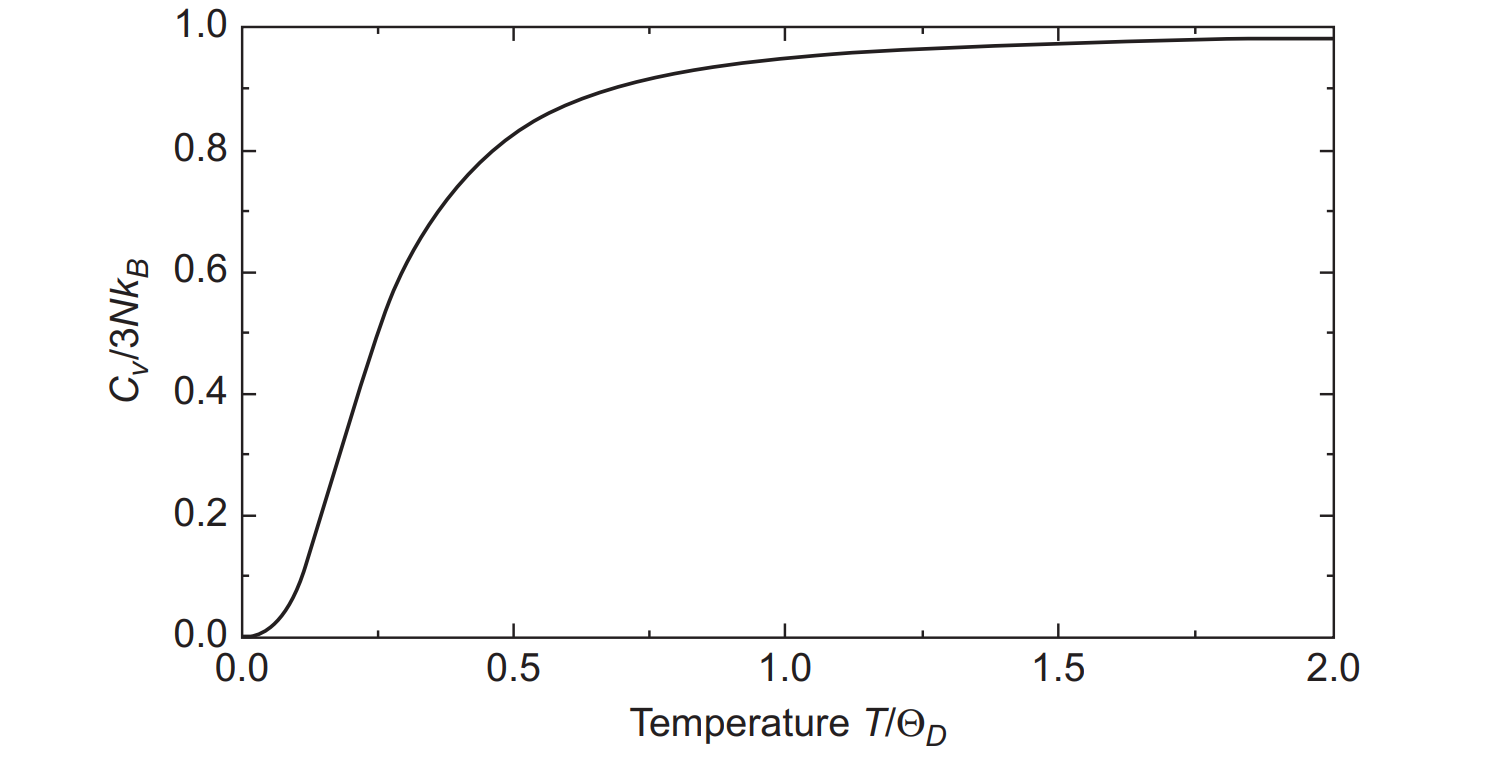
\includegraphics[width=0.8\textwidth]{fig/specific heat.png}
       \caption{晶体热容和温度的关系 \protect\footnotemark }
       \label{fig:specific heat with T}
\end{figure}
\footnotetext{图片来自Physics of Condensed Matter, P.K. Misra}

我们将用声子来描述机械波,声子和上文讨论的光子都是玻色子,区别在于\begin{enumerate}
    \item 作为弹性介质中的机械振动,其频率存在上限(由于力学的限制);
    \item 与光波一定是横波不同,机械波也可以是纵波。
\end{enumerate}

现在我们考虑一个$N$个原子的体系,其具有$3N$个自由度,将势能在极小值点$\diffp{U}{{x_i}}=0$的附近展开,有\begin{equation}
    U=U_0 =\frac{1}{2} \sum_{i=1}^{3N} \sum_{j=1}^N \diffp*{U}{{x_i}{x_j}}{0} \delta x_i \delta x_j=\frac{1}{2} \sum_{i,j} k_{ij} x_i x_j
\end{equation}
体系的动能可以写作\begin{equation}
    T=\frac{1}{2} \sum_{i=1}^{3N} \frac{p_i^2}{m_i}
\end{equation}
于是体系的哈密顿量为\begin{equation}
\begin{aligned}
    H&=T+V = \frac{1}{2} \sum_{i=1}^{3N} \frac{p_i^2}{m_i} +\frac{1}{2} \sum_{i,j} k_{ij} x_i x_j\\
    &=\frac{1}{2} \bd{p}^T M \bd{p} +\frac{1}{2}\bd{x}^T K \bd{x}
\end{aligned}
\end{equation}
其中\begin{equation}
    \bd{p}_{3N} =\begin{pmatrix}
        p_1\\
        p_2\\
        \vdots\\
        p_{3N}
    \end{pmatrix},\quad\bd{x}_{3N} =\begin{pmatrix}
        x_1\\
        x_2\\
        \vdots\\
        x_{3N}
    \end{pmatrix},\quad M= \begin{pmatrix}
        \frac{1}{m_1} & & \\
        & \ddots & \\
        & & \frac{1}{m_N}
    \end{pmatrix}_{3N\times 3N},\quad K= \begin{pmatrix}
        k_{1,1} & \cdots &k_{1,3N}\\
        \vdots & \ddots & \vdots\\
        k_{3N,1} & \cdots & K_{3N,3N}
    \end{pmatrix}
\end{equation}
其中$M$是一个对角阵,$K$是一个实对称方阵,它们一般无法同时直接对角化。采用质量权重变换:\begin{equation}
    \widetilde{p}_i = \frac{p_i}{\sqrt{m_i}} ,\quad \widetilde{x}_i =\sqrt{m_i} x_i,\quad[\widetilde{x}_i,\widetilde{p}_i]=i\hbar \delta_{ij},\quad \widetilde{k}_{ij} =\frac{k_{ij}}{\sqrt{m_i,m_j}}
\end{equation}
于是\begin{equation}
    H=\frac{1}{2} \bd{p}^T \cdot \bd{p}+\frac{1}{2} \widetilde{\bd{x}}^T\widetilde{K} \widetilde{\bd{x}}
\end{equation}
这个时候,存在$S^T S=1$满足,\begin{equation}
    S^T \widetilde{K} S=\Lambda
\end{equation}
其中$\Lambda=\mathrm{diag}(\lambda_1,\lambda_2,\cdots,\lambda_{3N})$
设\begin{equation}
    \widetilde{\bd{x}}=SQ,\quad \widetilde{\bd{p}}=SP
\end{equation}
从而得到\begin{equation}
\begin{aligned}
    H&=\frac{1}{2}\bd{p}^T \cdot \bd{p} +\frac{1}{2}Q^T \Lambda Q\\
    &=\sum_{i=1}^{3N} \left(p_k^2 +\lambda_k Q_k^2\right)\\
    &=\sum_{i=1}^{3N} h_k    
\end{aligned}
\end{equation}
其中$h_k=\frac{1}{2}(p_k^2+\lambda_k Q_k^2),\,\lambda_k=\omega_k^2\ge 0$。所以体系的哈密顿量可以分解为$3N$个部分,每个部分都是一个简谐振动。

对于每一个简谐振子,其能级分布为\begin{equation}
    \varepsilon_k(n_k)=(n_k+\frac{1}{2}) \hbar \omega_k
\end{equation}
我们可以将体系看作大量的声子组成的气体(phonon gas),每一个声子有$3N$种状态,第$k$个态的能量为$\varepsilon_k=\hbar \omega_k$,声子是一种玻色子,第$k$个态的占据数为$n_k$。

和光子气类似,声子也是全同粒子,并且总数不可确定,即其化学势是无意义的($\mu=0$)。类似地,我们可以将某一个微观态看作一组占据数:\begin{equation}
    v \leftrightarrow \{n_k\}
\end{equation}
每个状态对应的能量为\begin{equation}
    E_v =\sum_k (n_k +\frac{1}{2}) \hbar \omega_k
\end{equation}

我们可以对$3N$个可以区分的谐振子使用正则配分函数:\begin{equation}
    Q=\sum_v e^{-\beta E_v} =\prod_k Q_k
\end{equation}
其中$Q_k$是单谐振子配分函数,满足\begin{equation}
    Q_k =\sum_{n_k=0}^{\infty} e^{-\beta (n_k +\frac{1}{2})\hbar \omega_k} =\frac{e^{-\frac{1}{2}\beta \hbar \omega_k}}{1-e^{-\frac{1}{2}\beta \hbar \omega_k}}
\end{equation}

因此\begin{equation}
    \ln Q=\sum_k \ln \frac{e^{-\frac{1}{2}\beta \hbar \omega_k}}{1-e^{-\beta \hbar \omega_k}};
\end{equation}
根据正则系综中的结论:\begin{gather}
    \braket{E} =-\diffp{\ln Q}{\beta} =\sum_k \braket{\varepsilon_k(\omega_k)}    
\end{gather}
其中\begin{equation}
    \braket{\varepsilon_k(\omega_k)} =-\diffp{{\ln Q_k}}{\beta} =\frac{1}{2}\hbar \omega_k +\frac{1}{e^{\beta \hbar \omega_k}-1} \hbar \omega_k=(\braket{n_k}+\frac{1}{2}) \hbar \omega_k
\end{equation}

对于热容,我们有\begin{equation}
    C_V =\diffp{{\braket{E}}}{T} =\sum_k C_{V,k}
\end{equation}
其中\begin{equation}
\begin{aligned}
    C_{V,k}& =\diffp{\braket{\varepsilon_k}}{T} =-\frac{1}{k_B T^2} \diffp{\braket{\varepsilon_k}}{\beta}\\
    & =-\frac{\hbar\omega_k}{k_B T^2} \frac{-\hbar\omega_k e^{\beta\hbar\omega_k} }{\left(e^{\beta\hbar\omega_k}-1\right)^2}\\
    &=k_B (\beta\hbar\omega_k)^2 \frac{e^{\beta \hbar \omega_k}}{\left(e^{\beta\hbar\omega_k}-1\right)^2}
\end{aligned}
\end{equation}
记$\displaystyle \theta_k =\frac{\hbar \omega_k}{k_B}$,称为该振动模的振动特征温度\index{振动特征温度}。则有$\displaystyle \beta \hbar \omega_k=\frac{\theta_k}{T}$\begin{equation}
    C_{V,k} =k_B \left(\frac{\theta_k}{T}\right)^2 \frac{e^{\frac{\theta_k}{T}}}{(e^{\frac{\theta_k}{T}}-1)^2}
\end{equation}
不难发现$T\to+\infty$的时候,$C_{V,k}\to k_B$。

整个系统的热容,满足\begin{equation}
    C_V =\sum_k C_{V,k} =\int_0^{\omega_D} \di \omega g(\omega)C_V(\omega)
\end{equation}

类似前面的分析,在波矢空间中有\begin{equation}
    \rho(k)\di k =\frac{V}{2\pi^2} k^2 \di k
\end{equation}
并且$k=\frac{\omega}{c}$,注意到这个时候有两个横波自由度和一个纵波自由度\begin{equation}
    g(\omega)\di \omega =\frac{V}{2\pi^2} \left(\frac2{c_t^3}+\frac1{c_l^3}\right)\omega^2 \di \omega=A\omega^2 \di \omega
\end{equation}
我们知道有$3N$个简正模,因此\begin{equation}
    3N =\int_0^{\omega_D} g(\omega)\di \omega =\frac{1}{3}A \omega_D^3
\end{equation}
所以有$\displaystyle A=\frac{9N}{\omega_D^3}$。进而我们就可以计算热容\begin{equation}
    C_V =\int_0^{\omega_D} A\omega^2 k_B \left(\frac{\hbar\omega}{k_BT}\right)^2 \frac{e^{\frac{\hbar\omega}{k_BT}}}{\left(e^{\beta\hbar\omega_k}-1\right)^2}\di \omega^2
\end{equation}
做一个变量代换$\displaystyle x=\frac{\theta_k}{T}$就可以得到\begin{equation}
    C_V =9N k_B  \left(\frac{\hbar\omega_D}{k_BT}\right)^{-3}\int_0^{ \frac{\hbar\omega_D}{k_BT}} x^4 \frac{e^x}{(e^x-1)^2} \di x 
\end{equation}
令$\theta_D =\frac{\hbar\omega_D}{k_B}$。对于高温情形,$T\gg \theta_k$,所以$x\ll 1$,这个时候\begin{equation}
    C_V =9N k_B \left(\frac{\hbar\omega_D}{k_BT}\right)^{-3}\int_0^{ \frac{\theta_D}{T}}x^2 \di x  = 3N k_B 
\end{equation}

对于低温情形,$T\to 0$,$\theta_D\to \infty$,由\begin{equation}
    \int_{0}^{+\infty}\frac{x^4e^x}{(e^x-1)^2} \mathrm{d}x = \frac{4\pi^4}{15}
\end{equation}
所以\begin{equation}
    C_V =\frac{12}{5}\pi^4 N K_B \left(\frac{T}{\theta_D}\right)^3 \propto T^3 \label{equ:C_V in crystal}
\end{equation}

于是,我们就基本上解释了图\ref{fig:specific heat with T}所反映的物理现象。
% subsection 声子 (end)
% section photon_and_phonon (end)
\section{经典理想气体} % (fold)
\label{sec:经典理想气体}
\subsection{平动拆分} % (fold)
\label{sec:平动拆分}
事实上,单粒子的配分函数还可以进一步因子化,最常见的做法就是将平动的能级拆分出来\begin{equation}
    \varepsilon=\varepsilon_t+\varepsilon_{in}\Rightarrow q=q_t\cdot q_{in}
\end{equation}
其中$\varepsilon_t$和$q_t$是平动部分,$\varepsilon_{in}$和$q_{in}$是内部能量部分,进一步地,内部能量可以被拆分为核部分和其他部分(包括电子、振动、转动等)。即有\begin{equation}
    q=q_t q_n q_{\mathrm{other}}
\end{equation}
于是总的正则配分函数为\begin{equation}
\begin{aligned}
    \ln Q& = N \ln\frac{q}{N} +N\\
    & =\boxed{ N\ln \frac{q_t}{N}+N }+N \ln q_n + N \ln q_{\mathrm{other}}
\end{aligned}
\end{equation}
其中框内的部分都看作平动部分,框外的部分是分子内部结构的贡献。
% subsection 平动拆分 (end)
\subsection{无结构经典理想气体} % (fold)
\label{sub:无结构经典理想气体}
当气体分子没有内部结构的时候,只需要考虑平动的贡献。三维势箱中的一个粒子满足\begin{equation}
    \varepsilon(n_x,n_y,n_z)=\frac{h^2}{8mL^2} (n_x^2+n_y^2+n_z^2),\quad n_x,n_y,n_z=1,2,...
\end{equation}
某一个能级的态密度为\begin{equation}
    g(\varepsilon)\di \varepsilon =\frac{V}{4\pi^2}\cdot \frac{(2m)^{3/2}}{\hbar^3} \varepsilon^{1/2}\di \varepsilon
\end{equation}

从而平动配分函数为\begin{equation}
    q_t = \sum_i e^{-\beta \varepsilon_i} =\int_{0}^{+\infty} \rho(\varepsilon) e^{-\beta\varepsilon} \mathrm{d}x= \left(\frac{2\pi m k T}{h^2}\right)^{3/2} V =\frac{V}{\lambda^3}
\end{equation}

\begin{definition}
    上式中$\displaystyle \lambda=\sqrt{\frac{h^2}{2\pi m k T}}$被称为热波长\index{热波长}(Thermal wave length)。
\end{definition}
% subsection 无结构经典理想气体 (end)
\subsection{单原子和双原子理想气体分子} % (fold)
\label{sub:单原子和双原子理想气体分子}
\subsubsection{电子与核运动的分离}
对于单原子分子,原子内部的贡献仅限于核和电子。一个单原子分子的配分函数为\begin{equation}
    q=q_t q_n q_e
\end{equation}
其中原子核的部分可以写作$q_n=g_n^{(0)}e^{-\beta \varepsilon^{(0)}}=2I +1$,$I$是原子核的总自旋量子数。电子的部分可以写作\begin{equation}
\begin{aligned}
    q_e &=g_0^{(e)} e^{-\beta \varepsilon_0^{(e)}}+g_1^{(e)} e^{-\beta \varepsilon_1^{(e)}}+\cdots \\
    &=    e^{-\beta \varepsilon_0^{(e)}}\left(g_0^{(e)}+g_1^{(e)} e^{-\beta \delta \varepsilon_{10}^{(e)}}+\cdots\right)
\end{aligned}
\end{equation}
其中$\varepsilon_{j0}^{(e)}$是电子激发能,$g_j^{(e)}=2J+1$,$J$是该电子态的总角动量量子数。

在处理双原子分子的时候,我们首先需要假设核与电子的运动可以分离(这个近似被称为波恩-奥本海默近似\index{波恩奥本海默近似}或者绝热近似\index{绝热近似}):因为电子的运动速度比原子核快非常多,对于每一个电子态,可以认为核近似不动,对于原子核,可以认为电子形成了一个稳定的势场。

核的哈密顿量可以写成\begin{equation}
    H= K+V(R)
\end{equation}
其中动能$K=\frac{1}{2}(m_1 \dot{\bd{r}}_1^2 +m_2 \dot{\bd{r}}_2^2)$,在质心系中可以写成$K =\frac{1}{2}(M \dot{\bd{r}}_c^2 +\mu \dot{\bd{r}}^2)$。$\frac{1}{2}M \dot{\bd{r}}_c^2$的贡献纳入平动配分函数,因此核的哈密顿量只需要考虑相对运动项\begin{equation}
    \dot{\bd{r}}^2 =\dot{R}^2 + R^2 \dot\theta^2 +R^2 \sin^2\theta \dot\varphi^2
\end{equation}
所以\begin{equation}
    K=\frac{1}{2}\mu \left(\dot{R}^2 + R^2 \dot\theta^2 +R^2 \sin^2\theta \dot\varphi^2\right)
\end{equation}

\subsubsection{状态拆分}

双原子分子的配分函数可以拆分成核的贡献、分子内部结构的贡献和平动项的贡献。其中分子内部的贡献又可以进一步拆分成电子项、振动项和转动项。

我们对分子做完全解耦处理之后,配分函数就可以直接因子化。当电子的基态非常稳定的时候$\beta\Delta \varepsilon_{10}^{(e)}\gg 1$,所以\begin{equation}
    q_e\approx g_0^{(e)} e^{-\beta \varepsilon_0^{(e)}}
\end{equation}
对总配分函数的贡献只有一个因子,所以可以独立出来,即\begin{equation}
    q_{evr}=q_e q_{vr}
\end{equation}

\subsubsection{振动配分函数\index{振动配分函数}}
在声子气体中,\begin{equation}
    q_v =\frac{e^{-\beta \hbar \omega/2}}{1-e^{-\beta \hbar \omega}}=\frac{e^{-\frac12\frac{\theta_v}T}}{1-e^{-\frac{\theta_v}{T}}} =\begin{cases}
        \frac{T}{\theta_v}, & T\gg \theta_v\\
        e^{-\frac{\theta_v}{2T}},& T\ll \theta_v
    \end{cases}
\end{equation}
其中$\displaystyle \theta_v = \frac{\hbar\omega}{k_B}$被称为振动特征温度\index{振动特征温度},一般较大。而$\omega =\sqrt{\frac{k}{\mu}},k=\diffp*{U}{{R^2}}{0}$。
\subsubsection{转动配分函数\index{转动配分函数}}
对于一个刚性转子,我们有\begin{equation}
    \varepsilon_J = J(J+1)\frac{\hbar^2}{2I},\quad J=0,1,2,...,\ g_J=2J+1
\end{equation}
于是转动项对应的配分函数为\begin{equation}
    \begin{aligned}
        q_r &= \sum_{J=0}^{+\infty} (2J+1) e^{-J(J+1)\frac{\hbar^2}{2Ik_BT}}\\
        &= \sum_{J=0}^{+\infty} (2J+1) e^{-J(J+1)\frac{\theta_r}{T}}
    \end{aligned}
\end{equation}
其中$\displaystyle \theta_r=\frac{\hbar^2}{2I k_B}$被称为转动特征温度\index{转动特征温度},一般来说$\theta_r$比较小,可以作$\theta_r\ll T$近似。于是我们可以将求和转换成积分\begin{equation}
    q_r=\int_{0}^{+\infty} -\frac{T}{\theta_r}  \mathrm{d} e^{-J(J+1)\frac{\theta_r}{T}}=\frac{T}{\theta_r}
\end{equation}

\subsubsection{总配分函数}

综上,我们就得到了解耦近似下的所有配分函数,总配分函数为\begin{equation}
    q=\frac{q_n q_e q_t q_r q_v}{\sigma_{AB}}
\end{equation}
其中$\sigma$来自于经典的对称性或者量子力学熵的全同性原理,一般来说\begin{equation}
    \sigma_{AB} =\begin{cases}
        1 & A\neq B\\
        2 & A=B
    \end{cases}
\end{equation}
% subsection 单原子和双原子理想气体分子 (end)

\subsection{多原子分子气体} % (fold)
\label{sub:多原子分子气体}
多原子分子和双原子分子的分析方法是完全一致的,但是其自由度和配分函数会有一些不同。$N$原子分子会有$3N$个自由度,其中有三个平动自由度,线性分子有两个转动自由度,而非线性分子有三个转动自由度,剩下的自由度都属于振动自由度。
% subsection 多原子分子气体 (end)
% section 经典理想气体 (end)
\begin{review}
    \item 光的波粒二象性和黑体辐射;
    \item 声子和晶体的热容;
    \item 经典理想气体的平动拆分;
    \item 波恩奥本海默近似;
    \item 双原子分子的振动和转动配分函数;
\end{review}
\section{习题} % (fold)
\label{sec:习题5}

% section 习题 (end)
% chapter particles II (Application) (end)
%---------------------------------------------------------------------------